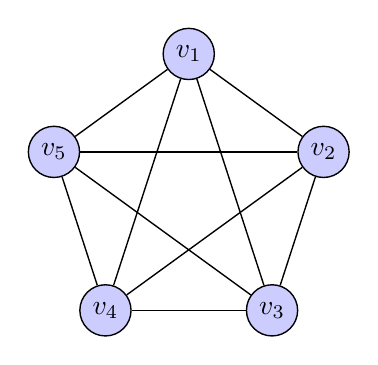
\begin{tikzpicture}[
  scale=1.0,
  vnode/.style={circle, fill=blue!20, draw=black, line width=0.5pt, inner sep=2pt, minimum size=6.5mm},
  edge/.style={line width=0.5pt, draw=black}
]

  % Vértices dispuestos en pentágono regular para máxima simetría
  \node[vnode] (v1) at (90:1.8) {$v_1$};
  \node[vnode] (v2) at (162:1.8) {$v_5$};
  \node[vnode] (v3) at (234:1.8) {$v_4$};
  \node[vnode] (v4) at (306:1.8) {$v_3$};
  \node[vnode] (v5) at (18:1.8) {$v_2$};

  % Todas las conexiones de un grafo completo K5 (10 aristas)
  \draw[edge] (v1) -- (v2);
  \draw[edge] (v1) -- (v3);
  \draw[edge] (v1) -- (v4);
  \draw[edge] (v1) -- (v5);

  \draw[edge] (v2) -- (v3);
  \draw[edge] (v2) -- (v4);
  \draw[edge] (v2) -- (v5);

  \draw[edge] (v3) -- (v4);
  \draw[edge] (v3) -- (v5);

  \draw[edge] (v4) -- (v5);

\end{tikzpicture}
